\documentclass[aps, pre, reprint, amsmath, amssymb, superscriptaddress, floatfix]{revtex4-2}

\usepackage{graphicx}
\usepackage{bm}
\usepackage{dcolumn}
\usepackage{hyperref}
\usepackage{xcolor}

\begin{document}

\title{Statistical mechanics of the queen lattice gas:\\
Monte Carlo simulations and Poisson mean-field theory}

\author{Zong-Yue Liu}
\affiliation{Department of Physics, Nanjing University, Nanjing 210093, China}

\author{Lei Wang}
\affiliation{Institute of Physics, Chinese Academy of Sciences, Beijing 100190, China}

\date{\today}

\begin{abstract}
We investigate the queen lattice gas---a model in which $M$ queens
are placed on an $N \times N$ chessboard with pairwise repulsive
interactions along shared rows, columns, and diagonals---from the
perspective of statistical mechanics.  At unit filling ($M = N$), the
ground states are exactly the $Q(N)$ solutions of the classical
$N$-queens problem, whose entropy per queen is
$s_0 \approx \ln N - \gamma$ ($\gamma \approx 1.942$).
We derive the exact high-temperature energy $E/M \to 5/3$ and show
that it decomposes as $1/2 \times 2$ (rows and columns)
$+ 1/3 \times 2$ (diagonals), with each contribution traceable to
the Poisson occupancy statistics of independent attack lines.
Extensive Monte Carlo simulations with $10^8$ sweeps per temperature
point for $N = 8$--$128$ reveal that the specific heat per queen
$C_v/M$ converges to a universal function of $T$ as $N \to \infty$,
with a non-divergent peak $C_v^{\max}/M \approx 1.62$ at
$T^* \approx 0.237\,J$, establishing the absence of a thermodynamic
phase transition.  We construct a modified Poisson mean-field theory
based on independent attack-line statistics that yields an analytical
expression for the limiting $E/M(T)$ and $C_v/M(T)$, reproducing
the Monte Carlo specific heat to within $2\%$ for $T \ge 0.3\,J$.
The mean-field decomposition reveals that at the specific heat peak,
rows and columns contribute $\sim 67\%$ and diagonals $\sim 33\%$ of
the total.
A thermodynamic integration of $C_v/T$ from $T = \infty$ to $T = 0$
recovers the known ground-state entropy, providing a nontrivial
self-consistency check linking combinatorics, simulation, and
analytical theory.  At half filling ($M = N^2/2$), the energy scales as
$E \sim N^3$---fundamentally different from the $E \sim N$
scaling at unit filling---and the system exhibits self-averaging,
with per-queen energy fluctuations that vanish in the
thermodynamic limit.
\end{abstract}

\maketitle

%=====================================================================
\section{Introduction}
\label{sec:intro}
%=====================================================================

The $N$-queens problem---placing $N$ mutually non-attacking queens on
an $N \times N$ chessboard---is among the oldest combinatorial
problems in mathematics, dating back to the work of Bezzel in
1848~\cite{Bezzel1848}.  Despite its long history, the asymptotic
enumeration of solutions was resolved only recently.  Simkin~\cite{Simkin2022}
proved that the number of solutions $Q(N)$ satisfies
\begin{equation}
  Q(N) = \left((1 \pm o(1))\frac{N}{e^{\gamma}} \right)^N, \quad
  \gamma \approx 1.942,
  \label{eq:QN}
\end{equation}
building on the breakthrough of Bowtell and
Keevash~\cite{Bowtell2023} and earlier bounds by Luria and
Simkin~\cite{Luria2021}.  The constant $\gamma$ has been refined
numerically~\cite{Nobel2023}.  Equation~\eqref{eq:QN} yields a
ground-state entropy per queen
$s_0 = \lim_{N \to \infty} \ln Q(N)/N = \ln N - \gamma + o(1)$.

Throughout this paper we set $k_B = 1$, so that entropy is
dimensionless and temperature has units of energy.
Interestingly, the functional form $s_0 = \ln N - \gamma$ is
reminiscent of the Sackur--Tetrode entropy per particle for an
ideal gas, $s_{\rm gas} = \ln(A/N\lambda_{\rm th}^2) + 2$~\cite{Reif1965},
in that both have the structure ``$\ln$(phase space) $+$ constant.''
We discuss this formal similarity further in
Sec.~\ref{sec:entropy}, though we stress that the underlying
physics is different: the queens entropy arises from discrete
combinatorial constraints rather than continuous phase-space
integration.

The entropy can be understood through a hierarchy of constraints
with increasing stringency~\cite{Knuth2022}:
\begin{itemize}
  \item \textit{Free placement} (row constraint only):
    $\Omega = N^N$, $s = \ln N$.
  \item \textit{Permutation} (row + column):
    $\Omega = N!$, $s \approx \ln N - 1$.
  \item \textit{N-queens} (row + column + two diagonals):
    $\Omega \approx (N/e^\gamma)^N$, $s \approx \ln N - \gamma$.
\end{itemize}
The column constraint costs exactly one unit of entropy (the
Stirling correction); the two diagonal constraints together cost
$\gamma - 1 \approx 0.94$ units.

A natural question arises: can the finite-temperature thermodynamics
of the queens system be understood analytically?
We address this by embedding the $N$-queens problem in
a queen lattice gas with tunable
temperature~\cite{Zhang2009,Polson2024}, performing extensive Monte
Carlo simulations, and deriving a Poisson mean-field theory based on
independent attack-line statistics that provides an accurate
(within a few percent) analytical description of the thermodynamics.

The queen lattice gas also connects to the broader field of
constraint satisfaction problems (CSPs)~\cite{Mezard2009,Krzakala2007}:
the $N$-queens problem at unit filling sits precisely at the
satisfiability threshold ($M \le N$: solvable; $M > N$: conflicts
unavoidable), paralleling random $k$-SAT near its critical clause
density.

The remainder of this paper is organized as follows.
Section~\ref{sec:model} defines the model.
Section~\ref{sec:entropy} discusses the ground-state entropy and its constraint hierarchy.
Section~\ref{sec:highT} derives the high-temperature limit.
Section~\ref{sec:mc} presents Monte Carlo results for $M = N$.
Section~\ref{sec:mf} develops the mean-field theory.
Section~\ref{sec:half} treats the half-filling case $M = N^2/2$.
Section~\ref{sec:conclusions} concludes.


%=====================================================================
\section{Model}
\label{sec:model}
%=====================================================================

We consider an $N \times N$ square lattice with open boundary
conditions.  Each site $(i,j)$ ($i,j = 1,\ldots,N$) carries an
occupation variable $n_{ij} \in \{0,1\}$.  The Hamiltonian counts
mutually attacking queen pairs:
\begin{equation}
  H = J \sum_{\langle (i,j),(i',j') \rangle_{\rm attack}}
  n_{ij}\, n_{i'j'},
  \label{eq:H}
\end{equation}
where the sum runs over all pairs sharing a row ($i = i'$), column
($j = j'$), main diagonal ($i - j = i' - j'$), or anti-diagonal
($i + j = i' + j'$), and $J > 0$.  We set $J = 1$ throughout.

The lattice decomposes naturally into \textit{attack lines}: $N$ rows,
$N$ columns, $2N-1$ main diagonals, and $2N-1$ anti-diagonals.
Writing $n_\alpha$ for the number of queens on line $\alpha$, the
Hamiltonian takes the compact form
\begin{equation}
  H = \sum_{\alpha \in \mathcal{L}} \binom{n_\alpha}{2},
  \label{eq:H_lines}
\end{equation}
where $\mathcal{L}$ denotes the set of all $6N - 2$ attack lines and
$\binom{n}{2} = n(n-1)/2$ counts the number of attacking pairs on
each line.  This decomposition into line contributions is the
starting point for both the high-temperature calculation
(Sec.~\ref{sec:highT}) and the mean-field theory (Sec.~\ref{sec:mf}).

We work in the canonical ensemble with fixed particle number
$M = \sum_{ij} n_{ij}$ and use Kawasaki dynamics~\cite{Kawasaki1966}
(queen--vacancy exchange) with the Metropolis acceptance
criterion~\cite{Metropolis1953}.  One \textit{sweep} consists of $M$
attempted exchanges.  Statistical errors are estimated by jackknife
resampling with 200 bins~\cite{Efron1982}.  For the principal
results at $M = N$, we simulate $N = 8, 16, 32, 64, 100,
128$ with $10^8$ measurement sweeps per temperature point (318
temperatures spanning $T = 0.05$ to $400\,J$), preceded by
$2 \times 10^6$ thermalization sweeps, using 32 CPUs in parallel.
We verified ergodicity by running independent simulations from
multiple random initial configurations (seeds); all runs yielded
statistically consistent results for $E/M$ and $C_v/M$ at every
temperature, confirming that the Kawasaki dynamics explores the
configuration space adequately within our thermalization and
measurement windows.
The schematic of the model and the relevant length scales are shown in
Fig.~\ref{fig:schematic}.

\begin{figure}[t]
  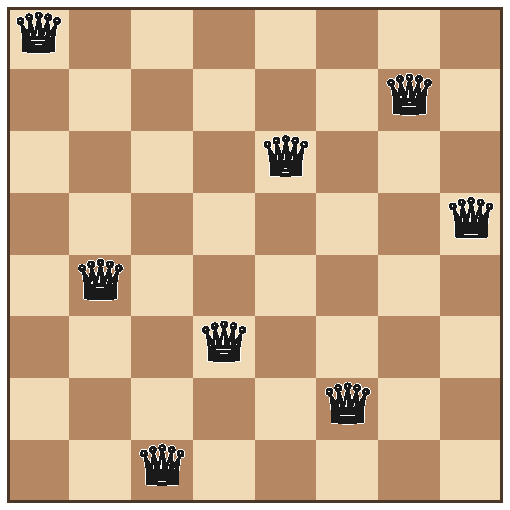
\includegraphics[width=\linewidth]{figures/fig1_schematic.pdf}
  \caption{(a)~A queen (black circle) and its four attack lines on an
  $8 \times 8$ board: row (red), column (blue), main diagonal
  (orange), anti-diagonal (purple).  (b)~One of the $Q(8) = 92$
  non-attacking configurations with $M = N = 8$ queens.  The board
  side $L = N\lambda$, where $\lambda$ is the lattice spacing (one
  cell width), defines the system size; $\ln N = \ln(L/\lambda)$
  gives the single-particle combinatorial entropy in the absence of
  column and diagonal constraints.}
  \label{fig:schematic}
\end{figure}


%=====================================================================
\section{Ground-state entropy and constraint hierarchy}
\label{sec:entropy}
%=====================================================================

For $M = N$ queens, the ground states ($E = 0$) correspond to the
$Q(N)$ non-attacking configurations.  Using
Eq.~\eqref{eq:QN}, the entropy per queen is
\begin{equation}
  s_0 = \frac{\ln Q(N)}{N}
  = \ln N - \gamma + o(1), \quad \gamma \approx 1.942.
  \label{eq:s0}
\end{equation}

The three-level constraint hierarchy (Table~\ref{tab:entropy_levels})
provides a physical interpretation.  Starting from a fully
unconstrained model where each queen independently chooses one of $N$
columns ($\Omega_{\rm free} = N^N$, $s_{\rm free} = \ln N$), the
column non-repetition constraint reduces the count to $N!$
permutations.  By Stirling's approximation,
$\ln N! = N\ln N - N + O(\ln N)$, so the entropy per queen is
\begin{equation}
  s_{\rm perm} = \frac{\ln N!}{N}
  = \ln N - 1 + O\!\left(\frac{\ln N}{N}\right).
  \label{eq:s_perm}
\end{equation}
Thus the column constraint costs exactly one unit of entropy---the
Stirling correction arising from the indistinguishability of column
assignments, exactly analogous to the Gibbs $1/N!$ factor in the ideal
gas~\cite{Reif1965}.

The two diagonal constraints further reduce the entropy to
$s_0 = \ln N - \gamma$, costing an additional $\gamma - 1 \approx
0.94$ units, or approximately $(\gamma - 1)/2 \approx 0.47$ units
per diagonal family.  The hierarchy of costs is physically natural:
the column constraint, being a global permutation on $N$ equivalent
lines, removes exactly one unit of freedom per queen, while each
diagonal family---whose lines have unequal lengths ranging from $1$
to $N$---removes roughly half a unit.

\begin{table}[b]
  \caption{Entropy per queen under successive constraints for the
  $N$-queens problem.  The column constraint costs exactly 1 unit;
  the two diagonal constraints cost $\gamma - 1 \approx 0.94$ units
  combined.}
  \label{tab:entropy_levels}
  \begin{ruledtabular}
  \begin{tabular}{llcc}
    Model & Constraints & $\Omega$ & $s = \frac{1}{N}\ln\Omega$ \\
    \hline
    Free & Row only & $N^N$ & $\ln N$ \\
    Permutation & Row + column & $N!$ & $\ln N - 1$ \\
    $N$-queens & Row + col + 2 diag & $\approx (N/e^\gamma)^N$
      & $\ln N - \gamma$ \\
  \end{tabular}
  \end{ruledtabular}
\end{table}

As noted in the introduction, the form $s_0 = \ln N - \gamma$ is
superficially similar to the 2D Sackur--Tetrode result
$s_{\rm gas} = \ln(A/N\lambda^2) + 2$: in both cases the entropy
takes the form ``$\ln$(accessible states) $+$ constant.''
However, this analogy should not be pushed too far.  The ideal gas
constant $+2$ arises from continuous momentum integration and the
Gibbs $1/N!$ correction, whereas $-\gamma$ encodes purely discrete
geometric exclusion constraints.  The resemblance is thus a formal
one, reflecting the common mathematical structure of counting
independent degrees of freedom reduced by constraints, rather than a
deep physical equivalence.


%=====================================================================
\section{High-temperature limit}
\label{sec:highT}
%=====================================================================

At $T \to \infty$, all $\binom{N^2}{M}$ configurations with $M$
queens are equally probable.  The exact high-temperature energy can be
obtained by linearity of expectation~\cite{Polson2024}: writing the
energy as a sum over all attacking site pairs, each pair is occupied
with probability $M(M-1)/[N^2(N^2-1)]$ (a combinatorial identity
independent of the pair's location).  Multiplying by the total number
of attacking site pairs $S_{\rm tot} = N(N-1)(5N-1)/3$---comprising
$N^2(N-1)/2$ from rows, the same from columns, and $N(N-1)(2N-1)/6$
from each diagonal family---yields the exact result for arbitrary $M$
and $N$:
\begin{equation}
  \frac{\langle E \rangle}{M}\bigg|_{T \to \infty}
  = \frac{(5N-1)(M-1)}{3N(N+1)}.
  \label{eq:E_highT_general}
\end{equation}
For the unit-filling case $M = N$, this reduces to
\begin{equation}
  \frac{\langle E \rangle}{M}\bigg|_{\substack{T \to \infty \\ M = N}}
  = \frac{(5N-1)(N-1)}{3N(N+1)}
  \xrightarrow{N \to \infty} \frac{5}{3}.
  \label{eq:E_highT}
\end{equation}

We now rederive the $N \to \infty$ limiting value $5/3$ by
decomposing the energy into line contributions, using a Poisson
approximation that reveals the physical origin of each term.

\subsection{Row and column contributions}

Consider the column contribution.  In a uniform random placement of
$M = N$ queens on $N^2$ sites, the expected number per column is
$M/N = 1$.  This is a classical \textit{balls-in-bins} problem:
$N$ balls (queens) distributed into $N$ bins (columns).  In the $N \to \infty$ limit,
the number of queens $n_c$ in any given column follows a Poisson
distribution with mean $\mu = M/N = 1$:
\begin{equation}
  P(n_c = k) = \frac{e^{-1}}{k!}, \quad k = 0, 1, 2, \ldots
  \label{eq:Poisson_col}
\end{equation}
The energy contributed by one column is $\binom{n_c}{2} =
n_c(n_c - 1)/2$.  Its expectation under the Poisson distribution is
\begin{equation}
  \left\langle \binom{n_c}{2} \right\rangle
  = \frac{1}{2}\bigl(\langle n_c^2 \rangle - \langle n_c \rangle\bigr)
  = \frac{1}{2}(\mu^2 + \mu - \mu) = \frac{\mu^2}{2} = \frac{1}{2},
  \label{eq:col_energy}
\end{equation}
where we used the Poisson identity $\langle n^2 \rangle = \mu^2 +
\mu$.  Summing over $N$ columns and dividing by $M = N$ gives a per-queen
column contribution of $1/2$; the row contribution is identical by
symmetry.

\subsection{Diagonal contributions}

For the diagonals, the argument is similar but the varying diagonal
lengths introduce an integral.  An $N \times N$ board has $2N - 1$
main diagonals of lengths $\ell = 1, 2, \ldots, N, \ldots, 2, 1$.
A diagonal of length $\ell$ passes through $\ell$ of the $N^2$ sites.
With $M = N$ queens placed uniformly at random, the mean number of
queens on this diagonal is $\mu_d = \ell \cdot M/N^2 = \ell/N$.
The expected collision energy per diagonal is
$\langle\binom{n_d}{2}\rangle = \mu_d^2/2 = \ell^2/(2N^2)$, using
the Poisson result.

Summing over all $2N - 1$ main diagonals and dividing by $M = N$:
\begin{equation}
  \frac{E_{\rm diag}^+}{M} = \frac{1}{N} \sum_{d}
  \frac{\ell_d^2}{2N^2}.
  \label{eq:E_diag_sum}
\end{equation}
For the $2N - 1$ main diagonals, the sum of squared lengths is
$\sum \ell_d^2 = 2\sum_{k=1}^{N-1} k^2 + N^2 = N(2N^2+1)/3$.
Thus
\begin{equation}
  \frac{E_{\rm diag}^+}{M}
  = \frac{1}{N} \cdot \frac{N(2N^2+1)}{6N^2}
  = \frac{2N^2+1}{6N^2}
  \xrightarrow{N \to \infty} \frac{1}{3}.
  \label{eq:E_diag_exact}
\end{equation}
Equivalently, in the continuum limit the diagonal lengths are
parametrized by $\mu = \ell/N \in (0, 1]$, with a density of states
$\rho(\mu) = 2N$ (two diagonals at distance $\mu$ from each corner).
The integral becomes
\begin{equation}
  \frac{E_{\rm diag}^+}{M}
  \to 2\int_0^1 \frac{\mu^2}{2}\,d\mu = \frac{1}{3}.
  \label{eq:E_diag}
\end{equation}
Including both diagonal families, we obtain
\begin{equation}
  \frac{E}{M}\bigg|_{T \to \infty}
  = \underbrace{\frac{1}{2} + \frac{1}{2}}_{\text{rows + columns}}
  + \underbrace{\frac{1}{3} + \frac{1}{3}}_{\text{diagonals}}
  = \frac{5}{3}.
  \label{eq:53}
\end{equation}

This decomposition is verified by Monte Carlo simulations
(Fig.~\ref{fig:energy}): at high $T$, $E/M$ converges to the
finite-$N$ exact value given by Eq.~\eqref{eq:E_highT}, which
itself approaches $5/3$ from below as $N$ increases, with
corrections of order $O(1/N)$.


%=====================================================================
\section{Finite-temperature Monte Carlo results for \texorpdfstring{$M = N$}{M=N}}
\label{sec:mc}
%=====================================================================

Figure~\ref{fig:energy} shows $E/M$ vs.\ $T$ for $N = 8$--$128$.
The curves for $N \ge 32$ are nearly indistinguishable, confirming
rapid convergence to the thermodynamic limit.

\begin{figure}[t]
  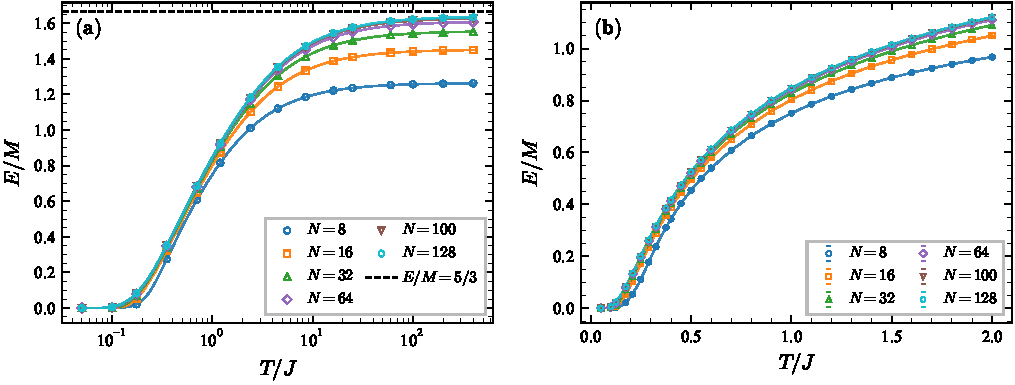
\includegraphics[width=\linewidth]{figures/fig2_energy.pdf}
  \caption{Energy per queen $E/M$ vs.\ temperature for
  $N = 8$--$128$.  (a)~Logarithmic temperature scale over the full
  range $T = 0.05$--$400\,J$; the dashed line marks the analytical
  $N \to \infty$ high-$T$ limit $E/M = 5/3$.  (b)~Linear scale,
  zoomed to $T \le 2\,J$, with error bars.}
  \label{fig:energy}
\end{figure}

\subsection{Specific heat convergence}

The specific heat per queen $C_v/M = (\langle E^2\rangle - \langle
E\rangle^2)/(T^2 M)$ is shown in Fig.~\ref{fig:cv}.  For $N \ge 32$,
the $C_v/M$ curves collapse onto a single function of $T$, indicating
that the thermodynamic limit has been reached.
Table~\ref{tab:cv_peak} lists the peak values.

\begin{figure}[t]
  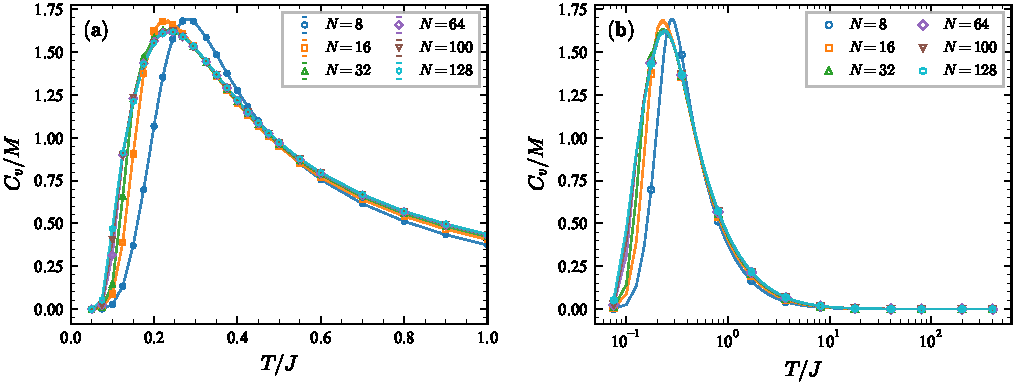
\includegraphics[width=\linewidth]{figures/fig3_cv.pdf}
  \caption{Specific heat per queen $C_v/M$ vs.\ $T$ for $M = N$.
  (a)~Peak region ($T \le 1\,J$, linear scale) with error bars.
  (b)~Full temperature range on a logarithmic $T$ scale.
  The curves for $N \ge 32$ collapse onto a single function,
  confirming convergence to the thermodynamic limit.}
  \label{fig:cv}
\end{figure}

\begin{table}[b]
  \caption{$C_v/M$ peak scaling for $M = N$, obtained by
  quartic polynomial fitting with bootstrap resampling (5000 samples).
  The peak height saturates near 1.62 for $N \ge 32$, ruling out a
  divergent susceptibility and hence a continuous phase transition.}
  \label{tab:cv_peak}
  \begin{ruledtabular}
  \begin{tabular}{rD{.}{.}{3}D{.}{.}{4}D{.}{.}{4}}
    $N$ & \multicolumn{1}{c}{$T_{\rm peak}$}
    & \multicolumn{1}{c}{$C_v^{\max}/M$}
    & \multicolumn{1}{c}{error} \\
    \hline
    8   & 0.281 & 1.6915 & 0.0002 \\
    16  & 0.227 & 1.6783 & 0.0006 \\
    32  & 0.231 & 1.6288 & 0.0005 \\
    64  & 0.237 & 1.6216 & 0.0004 \\
    100 & 0.237 & 1.6229 & 0.0004 \\
    128 & 0.237 & 1.6225 & 0.0004 \\
  \end{tabular}
  \end{ruledtabular}
\end{table}

The key observation is that $C_v^{\max}/M$ saturates near $1.62$ for
$N \ge 32$ and does \emph{not} diverge with system size.  This rules
out a thermodynamic phase transition and identifies the crossover as a
Schottky-type anomaly~\cite{Binder2010}---a broad peak in $C_v$
arising from thermal excitation across a finite energy gap, without
any symmetry breaking.  The peak temperature $T^* \approx 0.237\,J$
stabilizes for $N \ge 64$, and the peak height converges
monotonically from above: the residual finite-size correction
between $N = 64$ and $N = 128$ is only $\Delta C_v^{\max}/M
\approx 0.001$, well within the statistical error bars.

\subsection{Entropy self-consistency}
\label{sec:entropy_check}

The convergence of $C_v/M$ to a definite function enables a powerful
thermodynamic self-consistency check.  We compute the entropy
difference between $T = \infty$ and $T = 0$ in two independent ways.

\textit{Combinatorial route.}---At $T \to \infty$, all configurations
are equally probable, so the entropy per queen is
\begin{equation}
  \frac{S(\infty)}{N}
  = \frac{1}{N}\ln\binom{N^2}{N}.
  \label{eq:Sinf_def}
\end{equation}
For $N \ll N^2$, applying the Stirling approximation
$\ln n! = n\ln n - n + \tfrac{1}{2}\ln(2\pi n) + O(n^{-1})$:
\begin{align}
  \ln\binom{N^2}{N}
  &= \ln(N^2!) - \ln N! - \ln(N^2 - N)! \notag\\
  &= N\ln N - (N^2{-}N)\ln(1{-}1/N)
  + \Delta_{\rm S},
  \label{eq:Sinf_stirling}
\end{align}
where the first two terms come from the $n\ln n - n$ part of Stirling's
formula and the correction
$\Delta_{\rm S} = \tfrac{1}{2}\ln[N^2/(2\pi N(N^2-N))]
= -\tfrac{1}{2}\ln(2\pi(N-1))$ collects the subleading logarithms.
Expanding $\ln(1 - 1/N) = -1/N - 1/(2N^2) - \cdots$, the
leading terms give $-(N^2-N)\ln(1-1/N) = N - \tfrac{1}{2} + O(N^{-1})$,
so
\begin{equation}
  \frac{S(\infty)}{N}
  = \ln N + 1 + O\!\left(\frac{\ln N}{N}\right).
  \label{eq:Sinf}
\end{equation}
At $T = 0$, only ground states contribute:
$S(0)/N = \ln Q(N)/N \approx \ln N - \gamma$.

\textit{Thermodynamic route.}---The fundamental relation
\begin{equation}
  S(\infty) - S(0) = \int_0^\infty \frac{C_v}{T}\,dT
  \label{eq:thermo_int}
\end{equation}
relates the entropy difference to the specific heat.  Dividing by $N$
and substituting the results above:
\begin{equation}
  \int_0^\infty \frac{C_v}{NT}\,dT
  = \frac{S(\infty) - S(0)}{N}
  = 1 + \gamma + O\!\left(\frac{\ln N}{N}\right)
  \approx 2.94.
  \label{eq:DS}
\end{equation}
This is a remarkable relation: the left side involves $C_v(T)$ measured by simulation over the entire
temperature range, while the right side involves only the
\emph{combinatorial} constants 1 (from the Stirling correction) and
$\gamma$ (from the Simkin asymptotic formula).

Rearranging Eq.~\eqref{eq:DS}, we can extract the ground-state
entropy per queen directly from the Monte Carlo data:
\begin{equation}
  s_0^{\rm MC}
  = \frac{S(\infty)}{N} - \int_0^\infty \frac{C_v}{NT}\,dT,
  \label{eq:s0_MC}
\end{equation}
where $S(\infty)/N = \frac{1}{N}\ln\binom{N^2}{N}$ is exact.
This provides a purely thermodynamic determination of the
ground-state degeneracy without direct enumeration.

The numerical integration uses 318 temperature grid points
logarithmically spaced from $T = 0.05\,J$ to $400\,J$; the low-$T$
cutoff contributes negligibly since $C_v/T$ is exponentially
suppressed below $T \approx 0.1\,J$, and the high-$T$ cutoff at
$400\,J$ is sufficient because $C_v/T \propto T^{-3}$ decays
rapidly, contributing less than $0.01\%$ of the integral beyond
this point.  The trapezoidal rule on the logarithmic grid introduces
discretization errors well below the statistical uncertainty of the
Monte Carlo data.

Table~\ref{tab:entropy_check} summarizes the results.
For $N = 8$ and $N = 16$, where exact values of $Q(N)$ are known
($Q(8) = 92$, $Q(16) = 14\,772\,512$), $s_0^{\rm MC}$ agrees with
the exact $s_0^{\rm exact} = \ln Q(N)/N$ to within $1.2\%$ and
$0.5\%$ respectively, validating the simulation and integration
procedure.

For $N \ge 32$, where exact $Q(N)$ is unknown, we use $s_0^{\rm MC}$
to extract the Simkin constant via
$\gamma_{\rm MC} = \ln N - s_0^{\rm MC}$.
The extracted values converge monotonically toward the known
asymptotic value $\gamma = 1.942$~\cite{Simkin2022,Nobel2023}:
$\gamma_{\rm MC} = 1.83$ ($N = 32$), $1.89$ ($N = 64$),
$1.90$ ($N = 100$), $1.92$ ($N = 128$), with the deviation
decreasing from $5.9\%$ to $1.1\%$.
The dominant source of error at moderate $N$ is the finite-size
correction to the Simkin formula [the $o(1)$ term in
Eq.~\eqref{eq:QN}], which makes $\gamma_{\rm eff}(N)
= \ln N - s_0(N)$ systematically smaller than the asymptotic
$\gamma$; the MC integration itself introduces only sub-percent
errors, as confirmed by the $N = 8$ and $N = 16$ benchmarks.
The monotonic convergence of $\gamma_{\rm MC}$ toward $1.942$ with
increasing $N$ confirms the mutual consistency of the Monte Carlo
thermodynamics, the Stirling approximation for $S(\infty)$, and the
Simkin combinatorial formula.

\begin{table}[b]
  \caption{Ground-state entropy from thermodynamic integration.
  $s_0^{\rm MC} = S(\infty)/N - \int_0^\infty (C_v/NT)\,dT$, where
  $S(\infty)/N = \frac{1}{N}\ln\binom{N^2}{N}$ is exact.
  For $N \le 16$, $s_0^{\rm MC}$ is compared with the exact
  ground-state entropy $s_0^{\rm exact} = \ln Q(N)/N$.
  For $N \ge 32$, we extract
  $\gamma_{\rm MC} = \ln N - s_0^{\rm MC}$ and compare with the
  Simkin asymptotic value $\gamma = 1.942$.}
  \label{tab:entropy_check}
  \begin{ruledtabular}
  \begin{tabular}{cD{.}{.}{3}D{.}{.}{3}D{.}{.}{3}c}
    $N$ & \multicolumn{1}{c}{$s_0^{\rm MC}$}
    & \multicolumn{1}{c}{$s_0^{\rm exact}$}
    & \multicolumn{1}{c}{$\gamma_{\rm MC}$}
    & Deviation \\
    \hline
    8   & 0.558 & 0.565 & \multicolumn{1}{c}{---} & 1.2\% \\
    16  & 1.027 & 1.032 & \multicolumn{1}{c}{---} & 0.5\% \\
    \hline
    32  & 1.639 & \multicolumn{1}{c}{---} & 1.827 & 5.9\% \\
    64  & 2.268 & \multicolumn{1}{c}{---} & 1.891 & 2.6\% \\
    100 & 2.704 & \multicolumn{1}{c}{---} & 1.901 & 2.1\% \\
    128 & 2.931 & \multicolumn{1}{c}{---} & 1.921 & 1.1\% \\
  \end{tabular}
  \end{ruledtabular}
\end{table}

%=====================================================================
\section{Mean-field theory}
\label{sec:mf}
%=====================================================================

\subsection{Physical picture}

The decomposition of $H$ into line contributions
[Eq.~\eqref{eq:H_lines}] suggests a natural mean-field
approximation: treat the occupation numbers on different attack lines
as statistically independent.  In the dilute limit $M = N$, the
density $\rho = M/N^2 = 1/N \to 0$, and each queen belongs to four
lines that share no other queen with probability $1 - O(1/N)$.  The
correlation between any \emph{single pair} of attack lines is
therefore $O(1/N)$ and individually negligible.

However, this does not make the approximation exact: each line of
length $O(N)$ shares exactly one site with $O(N)$ other lines, so the
\emph{cumulative} effect of these individually weak correlations is
\begin{equation}
  \frac{\delta E}{M}
  \sim \frac{O(N)\text{ lines} \times O(N)\text{ neighbors} \times O(1/N)\text{ per pair}}{N}
  = O(1).
  \label{eq:mf_error}
\end{equation}
The independent-line approximation thus yields an $E/M$ that deviates
from the true value by an $O(1)$ amount---numerically a few
percent---even in the $N \to \infty$ limit.  Despite this systematic
bias, the approximation captures the correct functional form and
provides a quantitatively useful description of the thermodynamics.

\subsection{Simple Poisson mean-field}

We first present a simple approximation inspired by
Ref.~\cite{Polson2024}.  Each queen interacts along four families of
attack lines (row, column, main diagonal, anti-diagonal), but these
families are not equally constraining: the entropy analysis of
Sec.~\ref{sec:entropy} shows that each row or column constraint
removes one unit of entropy per queen, while the two diagonal
constraints together remove $\gamma - 1 \approx 0.942$ units.
We therefore assign an \emph{entropy-weighted} effective number
of interaction directions,
\begin{equation}
  \nu_{\rm eff} = \underbrace{1 + 1}_{\text{row + column}}
  + \underbrace{(\gamma - 1)}_{\text{two diagonals}} = 1 + \gamma
  \approx 2.942.
  \label{eq:nu_eff}
\end{equation}
Treating each effective direction independently and assigning each
conflict a Boltzmann suppression
$e^{-J/(2T)}$ (the factor of 2 accounts for the pairwise energy being
shared between two queens), the mean-field energy per queen is
\begin{equation}
  \frac{E^{\rm MF}}{M}
  = \frac{(1+\gamma)(N-1)}{2N}\,e^{-1/(2T)}
  \xrightarrow{N \to \infty}
  \frac{1+\gamma}{2}\,e^{-1/(2T)},
  \label{eq:E_simple}
\end{equation}
yielding the specific heat
\begin{equation}
  \frac{C_v^{\rm MF}}{M} = \frac{dE/M}{dT}
  = \frac{1+\gamma}{4T^2}\,e^{-1/(2T)}.
  \label{eq:Cv_simple}
\end{equation}
Setting $dC_v/dT = 0$ gives the peak location $T^* = 1/4$ with
\begin{equation}
  \frac{C_v^{\max}}{M} = \frac{4(1+\gamma)}{e^2} \approx 1.593,
  \label{eq:Cv_peak_simple}
\end{equation}
within $1.4\%$ of the Monte Carlo value $1.615$ for $N = 128$.
The remaining discrepancy arises because two approximations
have partially compensating effects: the entropy-weighted
prefactor $1+\gamma \approx 2.942$---which underestimates the
full four-family contribution---is offset by the neglect of
inter-line correlations, which overestimates the energy.
This compensation is not accidental but reflects the
physical content of the entropy weighting, which effectively
absorbs part of the correlation effect into a reduced number
of effective interaction directions.

\subsection{Modified Poisson mean-field}

A more systematic treatment retains the full decomposition into
four families of attack lines (rows, columns, main diagonals,
anti-diagonals) and accounts for the varying diagonal lengths.
At finite temperature, the occupation number of a line with mean
$\mu$ (at $T = \infty$) follows the
\textit{modified Poisson distribution}---a Poisson distribution
reweighted by the Boltzmann factor of the intra-line interaction.

For a single attack line with fugacity $\lambda$ at inverse
temperature $\beta = 1/T$, the probability of finding $k$ queens is
\begin{equation}
  P(n = k) = \frac{\lambda^k}{k!}\,
  e^{-\beta\,k(k-1)/2}\Big/\,g(\lambda, \beta),
  \label{eq:modPoisson}
\end{equation}
where the normalizing partition function is
\begin{equation}
  g(\lambda, \beta) = \sum_{k=0}^\infty
  \frac{\lambda^k}{k!}\,e^{-\beta k(k-1)/2}.
  \label{eq:g_def}
\end{equation}
The fugacity $\lambda$ is determined self-consistently by the
constraint $\langle n \rangle = \mu$:
\begin{equation}
  \mu = \frac{\lambda}{g}\,\frac{\partial g}{\partial \lambda}
  = \sum_{k=0}^\infty k\,P(k).
  \label{eq:mu_constraint}
\end{equation}

The physical content of Eq.~\eqref{eq:modPoisson} is transparent:
the $\lambda^k/k!$ factor is the standard Poisson weight for $k$
particles on a line, and $e^{-\beta k(k-1)/2}$ suppresses
configurations with many collisions.  At $\beta = 0$ ($T \to \infty$),
$P(k)$ reduces to a standard Poisson distribution; at $\beta \to
\infty$ ($T \to 0$), only $k = 0$ and $k = 1$ survive, enforcing the
non-attacking constraint.

The expected collision energy per line is
\begin{equation}
  f(\mu, \beta) = \left\langle\binom{n}{2}\right\rangle
  = \frac{1}{2}\sum_{k=2}^{\infty} k(k-1)\,P(k).
  \label{eq:f_def}
\end{equation}

The per-queen energy in the thermodynamic limit is then
\begin{equation}
  \frac{E}{M}(T) = \underbrace{2\,f\!\left(1,\tfrac{1}{T}\right)
  }_{\rm rows + columns}
  + \underbrace{4\int_0^1 f\!\left(\mu,\tfrac{1}{T}\right)d\mu
  }_{\rm diagonals},
  \label{eq:E_MF}
\end{equation}
where the first term sums over $N$ rows and $N$ columns (each with
$\mu = 1$), and the integral accounts for $2 \times (2N-1)$ diagonals
with $\mu = \ell/N \in (0,1]$.

\subsection{Low-temperature approximation}

At low temperatures ($\beta \gg 1$), the partition function $g$ is
dominated by the first few terms.  Truncating at $k = 2$:
\begin{equation}
  g \approx 1 + \lambda + \frac{\lambda^2}{2}\,e^{-\beta}.
  \label{eq:g_trunc}
\end{equation}
Note that the $k = 2$ Boltzmann factor is $e^{-\beta \cdot 2(2-1)/2}
= e^{-\beta}$, since two queens sharing a line cost energy $J = 1$.
Imposing $\langle n \rangle = 1$ for the row/column contribution
gives $(\lambda^2/2)e^{-\beta} = 1$, hence
$\lambda = \sqrt{2}\,e^{\beta/2}$.
The row + column energy per queen is then
\begin{equation}
  \frac{E_{\rm rc}}{M} \approx \frac{2}{2 + \sqrt{2}\,e^{\beta/2}},
  \label{eq:Erc_approx}
\end{equation}
which has the form of a two-level Schottky function.  The
corresponding specific heat contribution is
\begin{equation}
  \frac{C_{v,\rm rc}}{M} \approx
  \frac{\sqrt{2}\,e^{\beta/2}}{(2 + \sqrt{2}\,e^{\beta/2})^2}
  \cdot \frac{1}{T^2}.
  \label{eq:Cv_rc_approx}
\end{equation}
This two-level (Schottky) approximation correctly captures the peak
shape and explains why the specific heat does not diverge: the
energy gap $\Delta$ is finite, so thermal excitation is always a
smooth crossover rather than a critical phenomenon.

\subsection{Comparison with Monte Carlo}

Figure~\ref{fig:mf} compares both mean-field predictions with Monte
Carlo data.  The modified Poisson theory systematically overestimates
$E/M$ by $2$--$7\%$ (larger at low $T$).
As discussed in Sec.~\ref{sec:mf}A, this bias is an $O(1)$
effect arising from inter-line correlations whose individual weakness
[$O(1/N)$ per pair] is compensated by the large number of correlated
pairs [$O(N^2)$].  The simple MF achieves comparable accuracy because the
entropy-weighted prefactor partially absorbs the correlation
effects neglected by both approaches.

For the specific heat, the simple MF gives
$C_v^{\max}/M = 4(1+\gamma)/e^2 \approx 1.593$ (1.4\% from MC at $N = 128$),
while the modified Poisson MF gives $1.692$ (4.8\% from MC).  Both
correctly predict the absence of a divergence and the Schottky shape.
The mean-field decomposition reveals that at the $C_v$ peak,
rows + columns contribute $\sim 67\%$ and diagonals $\sim 33\%$ of
the total specific heat.

Table~\ref{tab:mf_comparison} provides a detailed comparison at
selected temperatures for $N = 128$.

\begin{table}[b]
  \caption{Modified Poisson mean-field vs.\ Monte Carlo ($N = 128$).
  The systematic overestimate in $E/M$ is an $O(1)$ effect of
  inter-line correlations neglected by the independent-line
  approximation (see text).}
  \label{tab:mf_comparison}
  \begin{ruledtabular}
  \begin{tabular}{cD{.}{.}{5}D{.}{.}{5}cD{.}{.}{3}D{.}{.}{3}c}
    $T$ & \multicolumn{1}{c}{$E_{\rm MC}/M$}
    & \multicolumn{1}{c}{$E_{\rm MF}/M$}
    & $\Delta E$
    & \multicolumn{1}{c}{$C_{v,\rm MC}/M$}
    & \multicolumn{1}{c}{$C_{v,\rm MF}/M$}
    & $\Delta C_v$ \\
    \hline
    0.200 & 0.12064 & 0.12952 & 7.4\% & 1.554 & 1.646 & 5.9\% \\
    0.225 & 0.16034 & 0.17140 & 6.9\% & 1.615 & 1.692 & 4.8\% \\
    0.300 & 0.27974 & 0.29460 & 5.3\% & 1.520 & 1.550 & 2.0\% \\
    0.500 & 0.52559 & 0.54263 & 3.2\% & 0.973 & 0.976 & 0.3\% \\
    1.000 & 0.84800 & 0.86633 & 2.2\% & 0.436 & 0.439 & 0.7\% \\
  \end{tabular}
  \end{ruledtabular}
\end{table}

\begin{figure}[t]
  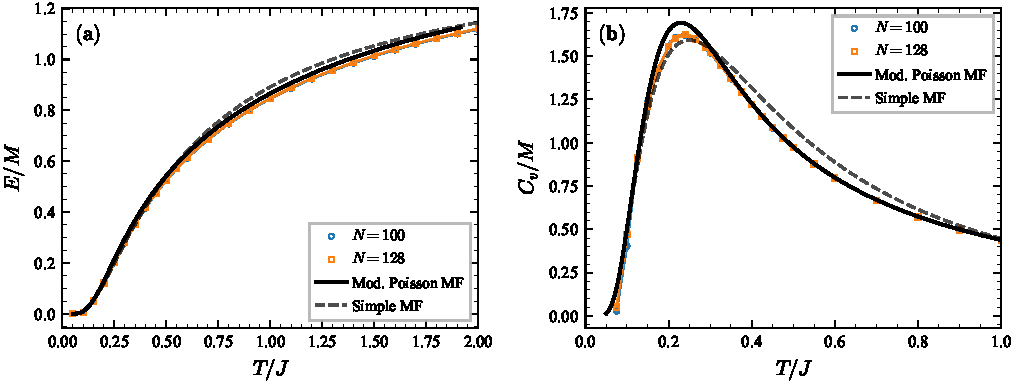
\includegraphics[width=\linewidth]{figures/fig4_meanfield.pdf}
  \caption{Mean-field theory vs.\ Monte Carlo for $M = N$.
  (a)~Energy per queen $E/M$ for $T \le 2\,J$; the solid curve is the
  modified Poisson MF [Eq.~\eqref{eq:E_MF}], the dashed curve is the
  simple MF.  (b)~Specific heat $C_v/M$ for $T \le 1\,J$; both MF
  curves reproduce the peak shape without any divergence.  Only
  $N = 100$ and $N = 128$ MC data are shown, as these are closest to
  the thermodynamic limit.}
  \label{fig:mf}
\end{figure}


%=====================================================================
\section{Half filling: \texorpdfstring{$M = N^2/2$}{M = N\^{}2/2}}
\label{sec:half}
%=====================================================================

We now turn to the opposite extreme of high density, setting
$M = N^2/2$.  This regime is fundamentally different from the dilute
$M = N$ case: each row contains on average $N/2$ queens, and the mean
number of queen pairs per line scales extensively with $N$.

\subsection{High-temperature energy scaling}

The high-temperature energy can be derived by the same
balls-in-bins decomposition as in Sec.~\ref{sec:highT}.  For
$M = N^2/2$ queens placed uniformly on $N^2$ sites, the mean
occupancy per row is $\mu_r = M/N = N/2$.  The expected collision
energy per row is $\langle\binom{n_r}{2}\rangle = \mu_r^2/2 = N^2/8$
(using the Poisson approximation, which is exact in the $N \to \infty$
limit when $M/N \to \infty$).  Summing over $N$ rows and dividing by
$M$ gives a per-queen row contribution of
$(N \cdot N^2/8)/(N^2/2) = N/4$.
Adding the column contribution (identical by symmetry) gives
$E_{\rm rc}/M = N/2$.

For the diagonals, a diagonal of length $\ell$ has mean occupancy
$\mu_d = \ell M/N^2 = \ell/2$.  Summing and taking the continuum
limit:
\begin{equation}
  \frac{E_{\rm diag}}{M}
  = \frac{4N}{M}\int_0^1 \frac{(N\mu/2)^2}{2}\,d\mu
  = \frac{4N \cdot N^2}{8 \cdot N^2/2}\int_0^1 \mu^2\,d\mu
  = \frac{N}{3}.
  \label{eq:E_half_diag}
\end{equation}
Combining:
\begin{equation}
  \frac{\langle E\rangle}{M}\bigg|_{T \to \infty}
  = \frac{N}{2} + \frac{N}{3} = \frac{5N}{6}.
  \label{eq:Ehalf}
\end{equation}
The subleading corrections give the exact result
$(5N - 6)/6 + O(N^{-1})$~\cite{Polson2024}.
The total energy $E = M \cdot (5N/6) \sim N^3$ makes this regime
fundamentally different from the dilute case ($E \sim N$).
Unlike the Ising model on a square lattice where $E \sim N^2$
(extensive in the number of sites), here the energy is
\emph{super-extensive} in $N^2$, reflecting the long-range nature of
the queen interaction.

\subsection{Self-averaging}

Figure~\ref{fig:half} shows the Monte Carlo results for
$N = 4$--$64$.  Two features are noteworthy.  First, the per-queen
energy $E/M$ increases proportionally to $N$
[Fig.~\ref{fig:half}(a)], consistent with
Eq.~\eqref{eq:Ehalf}.  Second, the specific heat peak narrows
and its per-queen magnitude decreases with $N$
[Fig.~\ref{fig:half}(b)], exhibiting \textit{self-averaging}.

Self-averaging is the phenomenon whereby macroscopic observables
become deterministic in the thermodynamic limit, familiar from
disordered systems~\cite{Mezard1987}.  In the queen lattice gas, it
arises because at half filling each queen interacts with $O(N)$ others
along its attack lines, making the per-queen energy a sum of many
correlated terms whose relative fluctuation vanishes with system size.
Quantitatively, the specific heat per queen $C_v/M$ decreases
monotonically with $N$ at fixed $T$---our Monte Carlo data at
$T = 0.3\,J$ give $C_v/M \approx 0.43$ ($N = 8$), $0.29$ ($N = 16$),
$0.16$ ($N = 32$), $0.089$ ($N = 64$)---and the relative energy
fluctuation per queen,
\begin{equation}
  \frac{\delta(E/M)}{E/M}
  = \frac{\sqrt{C_v T^2/M}}{E/M},
  \label{eq:self_avg}
\end{equation}
decreases rapidly with $N$, vanishing in the thermodynamic limit.
Thus each queen's energy becomes increasingly predictable as the
system grows, even though the total energy grows as $N^3$.  The
per-site specific heat $C_v/N^2 \to 0$ as $N \to \infty$: the
thermal fluctuations become negligible compared to the mean energy.

This contrasts sharply with the $M = N$ case, where
$C_v/M$ converges to a nonzero function.  The difference is that
at unit filling, each queen interacts with $O(1)$ others (on
average), so there is no self-averaging.

\begin{figure}[t]
  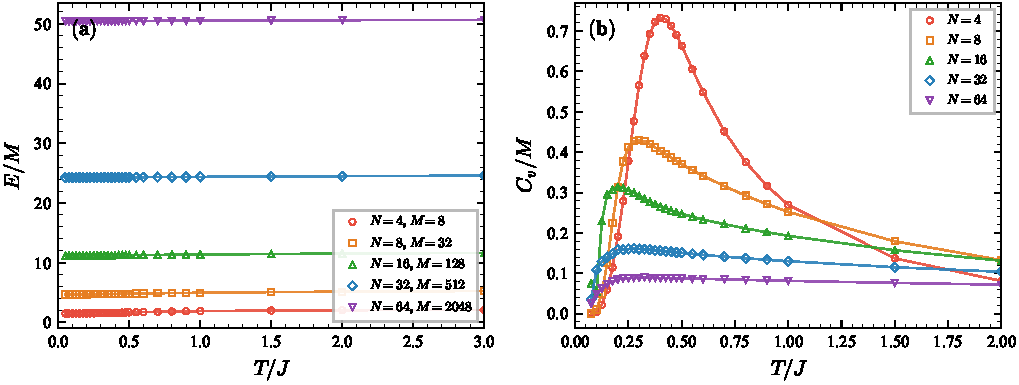
\includegraphics[width=\linewidth]{figures/fig5_halffilling.pdf}
  \caption{Half filling $M = N^2/2$.  (a)~Energy per queen $E/M$
  grows with $N$, scaling as $\sim 5N/6$.
  (b)~Specific heat per queen $C_v/M$: the peak narrows and
  the per-queen fluctuations decrease with $N$
  (self-averaging).  The contrast with the $M = N$ case
  (Fig.~\ref{fig:cv}), where $C_v/M$ converges, highlights
  the qualitative difference between the dilute and dense regimes.}
  \label{fig:half}
\end{figure}


%=====================================================================
\section{Conclusions}
\label{sec:conclusions}
%=====================================================================

We have presented a statistical-mechanical investigation of the queen
lattice gas, combining extensive Monte Carlo simulations with
analytical mean-field theory to characterize the finite-temperature
thermodynamics of the $N$-queens system.  Our main findings are:

\begin{enumerate}
\item The specific heat per queen $C_v/M(T)$ converges to a universal
  function of $T$ as $N \to \infty$.  The peak height $\approx 1.62$
  does not diverge, ruling out a thermodynamic phase transition and
  identifying the crossover as a Schottky anomaly with effective gap
  $\Delta = J$.

\item A modified Poisson mean-field theory, treating each attack line
  as an independent modified Poisson variable, provides an analytical
  expression for $E/M(T)$ and $C_v/M(T)$ that reproduces the Monte
  Carlo data to within $2$--$7\%$.  The residual bias is an $O(1)$
  systematic effect: each pair of attack lines is correlated at
  $O(1/N)$ through their shared lattice site, but the $O(N^2)$ such
  pairs produce a cumulative correction that persists in the
  $N \to \infty$ limit.  The simpler entropy-weighted MF
  [$C_v^{\max} = 4(1+\gamma)/e^2$] achieves $1.4\%$ accuracy at the
  peak because its entropy-weighted prefactor partially absorbs
  the correlation effects.

\item At $T \to \infty$, the energy per queen converges to
  $E/M = 5/3$, decomposing as $1/2 + 1/2 + 1/3 + 1/3$ from
  rows, columns, and two diagonal families.  Each contribution is
  derivable from Poisson occupancy statistics: $1/2 = \mu^2/2$ for
  lines with mean occupancy $\mu = 1$, and
  $1/3 = \int_0^1 \mu^2\,d\mu$ for diagonals with varying
  occupancy.

\item Thermodynamic integration of $C_v/T$ recovers the ground-state
  entropy per queen $s_0^{\rm MC} = S(\infty)/N - \int(C_v/NT)\,dT$,
  agreeing with exact values at $N = 8$ and $16$ to within $1.2\%$.
  For $N \ge 32$, the extracted Simkin constant
  $\gamma_{\rm MC} = \ln N - s_0^{\rm MC}$ converges monotonically
  to $\gamma = 1.942$, reaching $1.92$ at $N = 128$ ($1.1\%$
  deviation).  This nontrivial self-consistency check connects
  the Simkin combinatorial formula, the Stirling approximation for
  the high-temperature entropy, and the Monte Carlo specific heat
  data across the entire temperature range.

\item The ground-state entropy $s_0 = \ln N - \gamma$ can be
  decomposed through a constraint hierarchy: the column constraint
  costs exactly 1 unit of entropy per queen (the Stirling correction),
  while the two diagonal constraints together cost
  $\gamma - 1 \approx 0.94$ units.  This decomposition is formally
  reminiscent of the Sackur--Tetrode formula for an ideal gas,
  though the underlying mechanisms are distinct.

\item At half filling ($M = N^2/2$), $E \sim N^3$ and the system
  exhibits self-averaging: the per-queen specific heat $C_v/M$
  decreases with $N$, so relative energy fluctuations vanish in the
  thermodynamic limit.  This contrasts with the $M = N$ case where
  $C_v/M$ converges to a nonzero function, and reflects the
  extensive ($O(N)$) number of interactions per queen at high density.

\end{enumerate}

These results establish the queen lattice gas as a model system whose
thermodynamics can be quantitatively described by an independent
attack-line mean-field theory.  The analytical tractability
of the Poisson mean-field approach, the rich crossover
phenomenology between dilute and dense filling regimes, and the
interplay between combinatorial and thermodynamic quantities make
this model a compelling testbed for ideas at the interface of
constraint satisfaction and statistical mechanics.

Future directions include parallel tempering to access lower
temperatures, finite-size scaling theory for the Schottky crossover,
and replica overlap statistics to probe the solution space structure.


%=====================================================================
\begin{thebibliography}{30}

\bibitem{Bezzel1848}
M.~Bezzel,
Schachfreund, Berliner Schachzeitung \textbf{3}, 363 (1848).

\bibitem{Simkin2022}
M.~Simkin,
The number of $n$-queens configurations,
Adv.\ Math.\ \textbf{410}, 108735 (2022).

\bibitem{Bowtell2023}
C.~Bowtell and P.~Keevash,
The $n$-queens problem,
Ann.\ Math.\ \textbf{197}, 1 (2023).

\bibitem{Luria2021}
Z.~Luria and M.~Simkin,
New bounds on the number of $n$-queens configurations,
arXiv:2107.13460 (2021).

\bibitem{Nobel2023}
A.~Nobel, A.~Agrawal, and S.~Boyd,
Computing tighter bounds on the $n$-queens constant via Newton's
method,
Optim.\ Lett.\ \textbf{17}, 1229 (2023).

\bibitem{Reif1965}
F.~Reif,
\textit{Fundamentals of Statistical and Thermal Physics}
(McGraw-Hill, New York, 1965).

\bibitem{Knuth2022}
D.~E.~Knuth,
\textit{The Art of Computer Programming}, Vol.~4B
(Addison-Wesley, 2022), Sec.~7.2.2.

\bibitem{Zhang2009}
C.~Zhang and J.~Ma,
Counting solutions for the $N$-queens and Latin-square problems by
efficient Monte Carlo simulations,
Phys.\ Rev.\ E \textbf{79}, 016703 (2009).

\bibitem{Polson2024}
N.~Polson and V.~Sokolov,
Counting $N$ queens,
arXiv:2407.08830 (2024).

\bibitem{Mezard2009}
M.~M\'ezard and A.~Montanari,
\textit{Information, Physics, and Computation}
(Oxford University Press, Oxford, 2009).

\bibitem{Krzakala2007}
F.~Krzaka{\l}a, A.~Montanari, F.~Ricci-Tersenghi,
G.~Semerjian, and L.~Zdeborov\'a,
Gibbs states and the set of solutions of random constraint
satisfaction problems,
Proc.\ Natl.\ Acad.\ Sci.\ USA \textbf{104}, 10318 (2007).

\bibitem{Kawasaki1966}
K.~Kawasaki,
Diffusion constants near the critical point for time-dependent Ising
models.\ I,
Phys.\ Rev.\ \textbf{145}, 224 (1966).

\bibitem{Metropolis1953}
N.~Metropolis, A.~W.~Rosenbluth, M.~N.~Rosenbluth, A.~H.~Teller,
and E.~Teller,
Equation of state calculations by fast computing machines,
J.~Chem.~Phys.\ \textbf{21}, 1087 (1953).

\bibitem{Efron1982}
B.~Efron,
\textit{The Jackknife, the Bootstrap, and Other Resampling Plans}
(SIAM, Philadelphia, 1982).

\bibitem{Binder2010}
K.~Binder and D.~W.~Heermann,
\textit{Monte Carlo Simulation in Statistical Physics}
(Springer, Berlin, 5th ed., 2010).

\bibitem{Mezard1987}
M.~M\'ezard, G.~Parisi, and M.~A.~Virasoro,
\textit{Spin Glass Theory and Beyond}
(World Scientific, Singapore, 1987).

\end{thebibliography}

\end{document}
